\documentclass[14pt]{article}
\usepackage{geometry}
\usepackage[utf8]{inputenc}
\usepackage{cmap}
\usepackage[russian]{babel}
\usepackage{textcomp}
\usepackage{indentfirst}
\usepackage{amssymb}
\usepackage{graphicx}
\usepackage{lipsum}
\usepackage{setspace}
\usepackage{extsizes}
\usepackage{enumitem}
\usepackage{tabularx}
\usepackage{amsmath}
\usepackage{tocloft}
\usepackage{minted}
\usepackage[colorlinks=true,urlcolor=blue,linkcolor=]{hyperref}

% Пакет для объединения ячеек
\usepackage{multirow}
% Пакет для регуляции масштаба таблицы
\usepackage{tabularx}
% Пакет для работы с изображениями в документе
\usepackage{graphicx}
% Пакет для вставки кода (подсветка синтаксиса)
\usepackage{minted}
% Пакет для заголовков изображений\таблиц (для таблиц не обязателен)
\usepackage[font=small,labelfont=bf]{caption} 

\graphicspath{{images/}} 

\renewcommand{\cftsecleader}{\cftdotfill{\cftdotsep}}
\renewcommand{\cfttoctitlefont}{\LARGE\bfseries}
% Начало блока кода, который позволяет включить section* в оглавление
\usepackage{etoolbox}
\makeatletter
\newcommand\mysection[1]{%
	  \addcontentsline{toc}{section}{#1}%
	  \section*{#1}%
}
\makeatother

\makeatletter
\newcommand\mysubsection[1]{%
	  \addcontentsline{toc}{subsection}{#1}%
	  \subsection*{#1}%
}
\makeatother

\makeatletter
\newcommand\mysubsubsection[1]{%
	  \addcontentsline{toc}{subsubsection}{#1}%
	  \subsubsection*{#1}%
}
\makeatother
% Конец блока кода

\usepackage{titlesec}
\titleformat*{\section}{\LARGE\bfseries\centering}
\titleformat*{\subsection}{\Large\it}
\usepackage{pgfplots}

\newcolumntype{Y}{>{\centering\arraybackslash}X}

\begin{document}
\newgeometry{top=0.1in,bottom=0in,right=0.1in,left=0.1in}
\begin{spacing}{1}
\begin{center}
	\makebox[\linewidth][s]{МИНИСТЕРСТВО НАУКИ И ВЫСШЕГО ОБРАЗОВАНИЯ РОССИЙСКОЙ ФЕДЕРАЦИИ} \\
	\vspace{5mm}
	ФЕДЕРАЛЬНОЕ ГОСУДАРСТВЕННОЕ АВТОНОМНОЕ ОБРАЗОВАТЕЛЬНОЕ \\ УЧРЕЖДЕНИЕ ВЫСШЕГО ОБРАЗОВАНИЯ  \\
	\guillemotleft Национальный исследовательский университет ИТМО\guillemotright \\
	\vspace{5mm}
	ФАКУЛЬТЕТ ПРОГРАММНОЙ ИНЖЕНЕРИИ И КОМПЬЮТЕРНОЙ ТЕХНИКИ
	\vspace{60mm}
	
	{\bf \Large УЧЕБНО-ИССЛЕДОВАТЕЛЬСКАЯ РАБОТА №1} \\
	{ \large 
		\guillemotleft Обработка результатов измерений: статистический анализ \\
		числовой последовательности \guillemotright \\
		по дисциплине \\
		\guillemotleft Моделирование \guillemotright \\
		Вариант №28 \\
	}
\end{center}
\vspace{50mm}

\begin{flushright}
	{\it \textbf{Выполнил работу:}}\\
	Студент группы P3318 \\
	Рамеев Тимур Ильгизович \\
	{\it \textbf{Преподаватель:}}\\
	Авксентьева Елена\\
	Юрьевна\\
\end{flushright}
\vspace{5mm}
\end{spacing}
\begin{center}
    Санкт-Петербург  2024
\end{center}

\newgeometry{a4paper, top=0.5cm,bottom=3cm,right=1cm,left=1cm}
\newpage
\begin{center}
	\tableofcontents 
\end{center}
\setcounter{page}{1}

\sloppy

\newpage
\mysection{Цель}
	Изучение методов обработки и статистического анализа результатов измерений на примере заданной числовой последовательности путем оценки числовых моментов и выявления свойств последовательности на основе корреляционного анализа, а также аппроксимация закона распределения заданной последовательности по двум числовым моментам случайной величины.
\mysection{Выполнение}
\mysubsection{Расчет статистических характеристик заданной числовой последовательности}
	Для расчета оценки математического ожидания, оценки дисперсии, оценки СКО, доверительных интервалов, коэффициента вариации были использована следующие формулы расчета:

\begin{center}
	\large 
	$ \widetilde{m}= \frac{\sum^n_{i=1}X_i}{n} $
	\hspace{10mm}
	 $\widetilde{D}=\frac{\sum^n_{i = 1}(X_i - \widetilde{m})^2}{n - 1}$
\end{center}

	Среднее квадратическое отклонение (часто просто называемое стандартным отклонением) - это статистический показатель, который измеряет степень разброса значений в наборе данных относительно среднего значения. Среднее квадратическое отклонение дает представление о том, насколько близко значения в наборе данных сгруппированы вокруг среднего значения.

\begin{center}
	\large
	$\widetilde{\sigma}_m = \sqrt{\frac{\widetilde{D}}{n}}$
\end{center}

	Доверительный интервал - это интервал оценок для параметра генеральной совокупности, который строится на основе выборочных данных. Этот интервал задается таким образом, что с определенной заранее выбранной вероятностью (например - 95\%) истинное значение параметра генеральной совокупности попадает в этот интервал.

\begin{center}
	\large
	$\varepsilon_p = t_\alpha  \cdot \frac{\widetilde{\sigma}_m}{\sqrt{n}}$
\end{center}

	Коэффициент вариации - это статистический показатель, который измеряет относительную изменчивость (разброс) данных по отношению к их среднему значению.

\begin{center}	
	\large
	$v = \frac{\sigma}{m}$
\end{center}

\newpage

\begin{table}[h]
	\centering
	\caption{Характеристики заданной ЧП}
	\begin{tabularx}{\textwidth}{| c | c | X | X | X | X | X | X |}
		\hline
		Характеристика & & 10 & 20 & 50 & 100 & 200 & 300 \\
		\hline
		\multirow{2}{*}{Мат. ожидание} & Значение & 11,02  & 14,58  & 24,19  &  25,75 & 25,56 & \multirow{2}{*}{25,95} \\
		\cline{2-7}
		 & \% &  57,53 & 43,82 & 6,76 & 0,75  & 1,47  &   \\
		\hline
		\multirow{2}{*}{Дов. интервал (0,9)} & Значение & 4,06  & 5,55  & 7,61  &  6,34 & 4,37 & \multirow{2}{*}{3,65} \\
		\cline{2-7}
		 & \% & 11,18 & 52,11 & 108,45 & 73,71  & 19,68  & \\
		\hline
		\multirow{2}{*}{Дов. интервал (0,95)} & Значение  & 4,84  & 6,62 & 9,08 & 7,56 & 5,21 &  \multirow{2}{*}{4,35} \\
		\cline{2-7}
		 & \% & 11,18 & 52,11 & 108,45 & 73,71  & 19,68 &  \\
		\hline
		\multirow{2}{*}{Дов. интервал (0,99)} & Значение & 6,36 & 8,70 & 11,93 & 9,94 & 6,85 & \multirow{2}{*}{5,72} \\
		\cline{2-7}
		& \% & 11,18 & 52,11 & 108,45 & 73,71  & 19,68  & \\
		\hline
		\multirow{2}{*}{Дисперсия} & Значение & 61.00 & 228,35 & 1072,06 & 1489,05  & 1413,68 & \multirow{2}{*}{1480,35} \\
		\cline{2-7}
		 & \% &  95,88 & 84,57 & 27,58 & 0,59 & 4,50 & \\
		\hline
		\multirow{2}{*}{Ср. кв. отклонение} & Значение & 7,81 & 15,11 & 32,74  & 38,58 & 37,59 & \multirow{2}{*}{38,48} \\
		\cline{2-7}
		 & \% & 79,70 & 60,72 & 14,90 & 0,29 & 2,28 & \\
		\hline
		\multirow{2}{*}{К-т вариации} & Значение & 0,71 & 1,04 & 1,35 & 1,50 & 1,47 & \multirow{2}{*}{1,48} \\
		\cline{2-7}
		 & \% & 52,21 & 30,09 & 8,73 & 1.05 & 0,81 &  \\
		\hline
	\end{tabularx}
\end{table}
	\% - относительные отклонения рассчитанных значений от значений, полученных для выборки из трехсот величин.

	Приведенная выше таблица отражает полученные характеристики случайной последовательности. Полагается, что выборка из 300 чисел и рассчитанные для нее моменты являются эталонными.

	Если брать случайную выборку, то с увеличением размера выборки моменты будут меньше отклоняться от эталонных значений. Таким образом, увеличение размера выборки делает оценки статистик более надежными и близкими к истинными параметрам генеральной совокупности. Однако, стоит отметить, что бывают исключения - не всегда при росте выборки мы будем наблюдать более точные значения статистик. Наша таблица это наглядно демонстрирует.

\textbf{Оценка математического ожидания} показывает ожидаемое среднее значение случайной величины.

\textbf{Доверительный интервал} характеризует диапазон значений, в котором с определенной вероятностью находится случайная величина. Видно, что с увеличением доверительной вероятности доверительный интервал увеличивается - чем больше требование к вероятности попадания случайно величин в доверительный интервал, тем шире требуется интервал.

\textbf{Дисперсия и СКО} - характеризуют математическое ожидание отклонений от математического ожидания.

\textbf{Коэффициент вариации} - показывает отношение между мат. ожиданием отклонений и мат. ожиданием то есть то, насколько отклонение близко или далеко от мат. ожидания.

\newpage
\mysubsection{Построение графика значений для заданной числовой последовательности}
Обратимся к построенному графику значений заданной числовой последовательности.

\begin{center}
	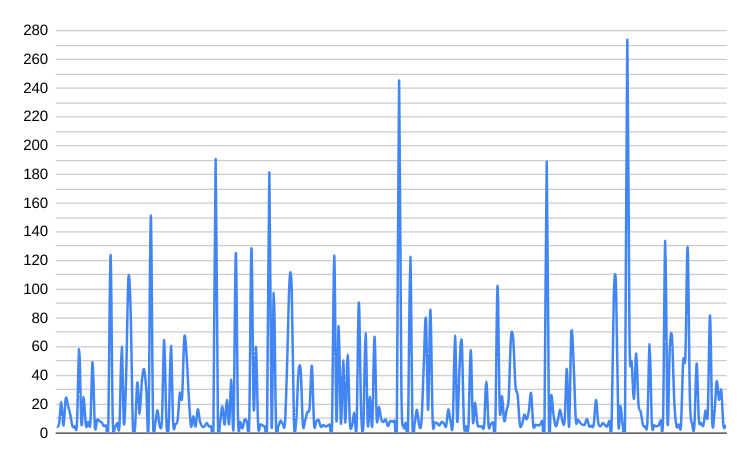
\includegraphics[scale=0.6]{graph_spec}
		\captionof{figure}{График значений заданной ЧП}
\end{center}

	Проанализировав данный график, можно сделать выводы о характере заданной числовой последовательности:
\begin{itemize}
	\item Не является возрастающей/невозрастающей
	\item Не является убывающей/неубывающей
	\item Не является периодической
\end{itemize}

Поскольку график значений для заданной числовой последовательности не имеет выраженных черт для данных характеристик.

\newpage
\mysubsection{Посроение гистограммы частот}
\begin{center}
	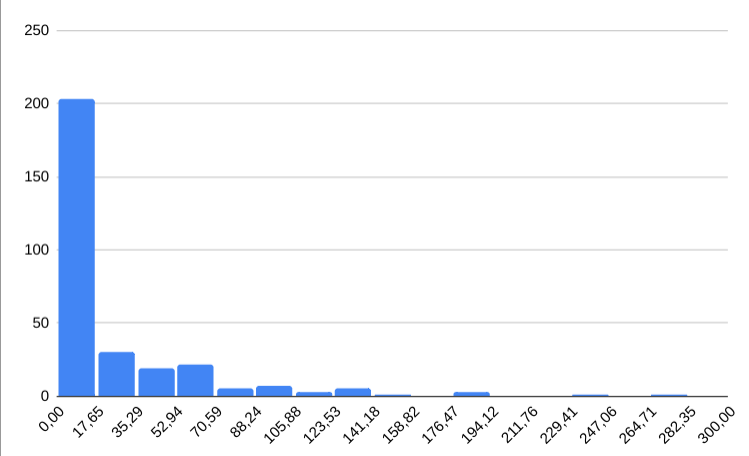
\includegraphics[scale=0.6]{hist_spec}
	\captionof{figure}{Гистограмма распределения частот заданной ЧП}
\end{center}

	Гистограмма дает представление функции плотности вероятности случайной величины, построенное по выборке. Можно сделать предположение, что заданная ЧП соответствует закону гиперэкспоненциального распределения.

	Гистограмма имеет длинный хвост, что означает наличие редких экстремальных значений в последовательности, что характерно для гиперэкспоненциального распределения. Это означает что при гиперэкспоненциальном распределении вероятность появления больших значений случайной величины значительно выше, чем, например, для экспоненциального распределения.

	Также гистограмма гиперэкспоненциального распределения по сравнению с экспоненциальным распределением характеризуется более резким спадом в области малых значений случайной величины, причем чем больше коэффициент вариации случайной величины, тем круче спад. Это значит, что вероятность появления маленьких значений случайной величины для гиперэкспоненциального распределения намного больше вероятности появления больших значений.
	
\newpage 

\mysubsection{Выполнение автокорреляционного анализа}
	Автокорреляция - это способ измерить, есть ли закономерность в последовательности. Она показывает, насколько текущее значение данных связано с предыдущими значениями, можно ли зная текущее значение, предсказать предыдущее/следующее.
	
\begin{table}[h]
	\small
	\centering
	\begin{tabularx}{\textwidth}{| c | X | X | X | X | X | X | X | X | X | X | }
		\hline
		Сдвиг ЧП & 1 & 2 & 3 & 4 & 5 & 6 & 7 & 8 & 9 & 10 \\
		\hline
		К-т АК для заданной ЧП & -0,0131 & 0,0069 & -0,0969 & -0,0948 & -0,0109 & 0,0051 & -0,0003 & -0,0002 & 0,0846 & 0,0226  \\
		\hline
	\end{tabularx}
\end{table}

	Коэффициенты автокорреляции заданной числовой последовательности для 9 сдвигов меньше 0.1, что позволяет сказать, что последовательность случайна.

\mysubsection{Выполнение аппроксимации закона распределения}

	Рассчитанный коэффициент вариации случайной величины $v = 1,48 > 1$

	Для аппроксимации закона распределения такой случайной величины используют \textbf{гиперэкспоненциальной распределение}, представляющее собой композицию экспоненциальных распределений.

	Стоит отметить, что аппроксимация гиперэкспоненциального распределения может осуществляться по трем моментам распределения, так как оно является трехпараметрическим, т.е. содержит три независимых параметра. Таким образом, имеется три параметра: q, t1, t2.

	По следующим формулам были рассчитаны три момента:

	Для аппроксимации закона распределения с коэффициентом вариации больше 1 двухфазным гиперэкспоненциальным распределением следует выбрать следующее значение вероятности:
	\begin{center}
		$q \leq \frac{2}{1 + v^2} = 0,62688 $
	\end{center}

	Пусть $ q = 0.6 $ (вероятность формирования значения случайной величины в первой фазе), тогда математические ожидания первой и второй экспоненциальных фаз будут равны соответственно рассчитанным t1 и t2:

	\begin{center}
		$t_1 = \left[1 + \sqrt{\frac{1 - q}{2q}(v^2 - 1)}\right] \cdot t = 42,348805$

		\vspace{0.5cm}

		$t_2 = \left[1 - \sqrt{\frac{q}{2(1 - q)}(v^2 - 1)}\right] \cdot t = 1,341817457$
	\end{center}

	Где t - математическое ожидание.


\newpage
\mysubsection{Реализация генератора случайных величин}

	Для реализации случайных величин в соответствии с законом гиперэкспоненциального распределения было решено воспользоваться тремя генераторами. Первые два экспоненциальные генераторы отвечают за фазы.  Третий генератор в свою очередь генерирует q-значение, от которого зависит, какая именно фаза сформирует сл. величину на данной итерации. Таким образом генерируем 300 значений величины, распределенной гиперэкспоненциально.

\begin{minted}[mathescape, linenos]{python}
	from scipy.stats import expon
	import random
	
	A1_value = 42.348805	
	A2_value = 1.341817457
	q_border = 0.6 # вероятность формирования сл. величины  в первой фазе
	VOLUME = 300
	
	
	def generate_values():
	    result_arr = []
	    for i in range(VOLUME + 1):
	        if random.random() >= q_border:
	            result_arr.append(expon.rvs(scale=A2_value, loc=0))
	        else:
	            result_arr.append(expon.rvs(scale=A1_value, loc=0))
	    return result_arr
	
	print(generate_values())
\end{minted}

\mysubsection{Генерация последовательности случайных величин}

	Была сгенерирована и проанализирована последовательность в соответствии гиперэкспоненциального распределения

	\newpage

\begin{table}[h]
	\centering
	\caption{Характеристики сгенерированной ЧП}
	\begin{tabularx}{\textwidth}{| c | c | X | X | X | X | X | X |}
		\hline
		Характеристика & & 10 & 20 & 50 & 100 & 200 & 300 \\
		\hline
		\multirow{2}{*}{Мат. ожидание} & Значение & 23,25&	30,26	&31,26	&30,59	&26,79	&26,92\\
		\cline{2-8}
		 & \% & 110,93	&107,56&	29,21	&18,80&	4,80	&3,74 \\
		\hline
		\multirow{2}{*}{Дов. интервал (0,9)} & Значение & 9,93	&14,74&	9,20	&6,51	&4,44	&3,63 \\
		\cline{2-8}
		 & \% & 144,73	&165,54	&20,88	&2,70	&1,61	&0,57\\
		\hline
		\multirow{2}{*}{Дов. интервал (0,95)} & Значение  & 11,85	&17,59	&10,97	&7,77	&5,29	&4,33  \\
		\cline{2-8}
		 & \% &  144,73&	165,54	&20,88&	2,70&	1,61&	0,57\\
		\hline
		\multirow{2}{*}{Дов. интервал (0,99)} & Значение & 15,57&	23,11&	14,42&	10,21	&6,96	&5,69 \\
		\cline{2-8} 
		& \% & 144,73	&165,54&	20,88	&2,70	&1,61	&0,57\\
		\hline
		\multirow{2}{*}{Дисперсия} & Значение & 365,32&	1 610,14	&1 566,56	&1 570,48&	1 459,65	&1 463,52 \\
		\cline{2-8}
		 & \% & 498,92&	605,12&	46,13&	5,47&	3,25	&1,14 \\
		\hline
		\multirow{2}{*}{Ср. кв. отклонение} & Значение &  19,11&40,13	&39,58&	39,63	&38,21&	38,26 \\
		\cline{2-8}
		 & \% & 144,73	&165,54	&20,88	&2,70	&1,61&	0,57 \\
		\hline
		\multirow{2}{*}{К-т вариации} & Значение &  0,82&	1,33&	1,27&	1,30	&1,43&	1,42 \\
		\cline{2-8}
		 & \% &  16,02	&27,93&	6,45&	13,55	&3,04	&4,15\\
		\hline
	\end{tabularx}
\end{table}
	
	\% - относительные отклонения характеристик сгенерированной случайной последовательности от одноименных значений заданной числовой последовательности

	Поскольку отклонения имеют малые значения для выборки из 300 чисел, можно утверждать, что сгенерированная последовательность близка по характеристикам к исходной.


\mysubsection{Автокорреляционный анализ сгенерированной последовательности}

	Коэффициенты автокорреляции сгенерированной числовой последовательности для всех сдвигов меньше 0.1, что позволяет сказать, что последовательность случайна.

	\begin{table}[h]
	\small
	\centering
		\begin{tabularx}{\textwidth}{| c | X | X | X | X | X | X | X | X | X | X | }
			\hline
			Сдвиг ЧП & 1 & 2 & 3 & 4 & 5 & 6 & 7 & 8 & 9 & 10 \\
			\hline
			К-т АК для заданной ЧП & -0,0131 & 0,0069 & -0,0969 & -0,0948 & -0,0109 & 0,0051 & -0,0003 & -0,0002 & 0,0846 & 0,0226  \\
			\hline
			К-т АК для сгенер. ЧП  & 0,0273 & -0,0629 & 0,0382 & -0,0388 & -0,0722 & -0,0234 & -0,0192 & -0,0452 & 0,0244 & 0,0392\\
			\hline
			\% & 147,95 & 110,96 & 353,68 & 144,21 & 84,91 & 121,74 & 98,51 & 99,51 & 246,30 & 42,32 \\
			\hline
	\end{tabularx}
	\end{table}

	Автокорреляционный анализ - это инструмент для изучения зависимостей внутри временных рядов. Он позволяет выявлять сохраняется ли зависимость между значениями временного ряда на различных лагах во времени.

\newpage
\mysubsection{Сравнительный анализ заданной и сгенерированной последовательностей}
	\begin{center}
		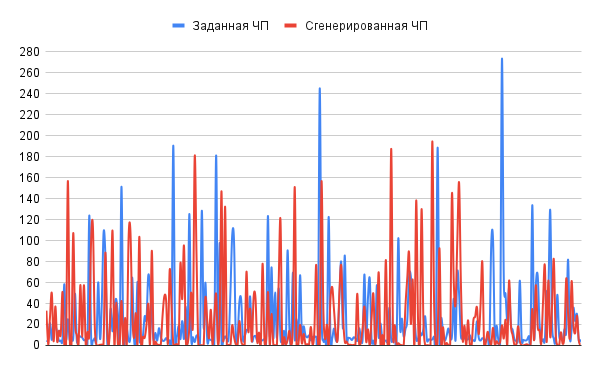
\includegraphics[scale=0.7]{graph_spec_gen}
		\captionof{figure}{График значений ЧП}
	\end{center}
	\begin{center}	
		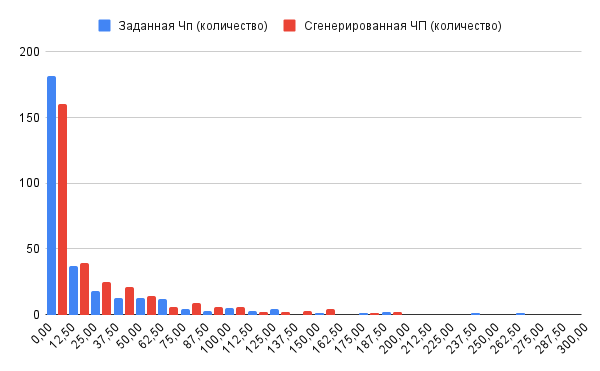
\includegraphics[scale=0.7]{hist_spec_gen}	
		\captionof{figure}{Гистограммы распределения частот}
	\end{center}
\newpage
\mysubsection{Оценка корреляционной зависимости заданной и сгенерированной последовательностей }

	Мы можем использовать функцию =КОРЕЛЛ(диапазон1; диапазон2), чтобы вычислить коэффициент корреляции между заданной и сгенерированной последовательностями данных. Результат расчета коэффициента корреляции для этих двух последовательностей составляет \textbf{-0,03324877454}.

	Это значение коэффициента корреляции невелико, что позволяет сделать вывод о том, что между числовыми последовательностями нет значительной зависимости или влияния друг на друга.

\mysection{Выводы}
	В рамках выполненной лабораторной работы было проведено исследование числовой последовательности. Анализ последовательности включал в себя оценку числовых моментов, а также корреляционный анализ для выявления ее особенностей. Кроме того, предпринимались попытки аппроксимации данной последовательности гиперэкспоненциальным законом распределения, основанным на трех числовых моментах случайной величины.

	Был написан код, генерирующий случайную последовательность чисел по закону гипреэкспоенециального распределения. В рамках сравнительного анализа статистических характеристик и графического представления данных были проведены сопоставления между исходной числовой последовательностью и сгенерированной последовательностью.

	На основе полученных результатов можно сделать вывод о том, что был выбран верный закон распределения для аппроксимации данной случайной величины. Это подтверждается тем,что оценки математического ожидания, доверительных интервалов и коэффициентов автокорреляции практически совпадают между исходной и сгенерированной последовательностями.

	Полученные результаты позволили углубиться в понимании основных статистических характеристик данных, что может быть полезным для более точного анализа и интерпретации данных в будущем.
\end{document}